\documentclass[tikz,border=5pt]{standalone}
\usepackage{tikz}
\usepackage{amsmath}
\usetikzlibrary{arrows.meta}
\definecolor{nebula}{HTML}{6366F1}
\definecolor{spark}{HTML}{14B8A6}
\definecolor{ink}{HTML}{334155}
\begin{document}
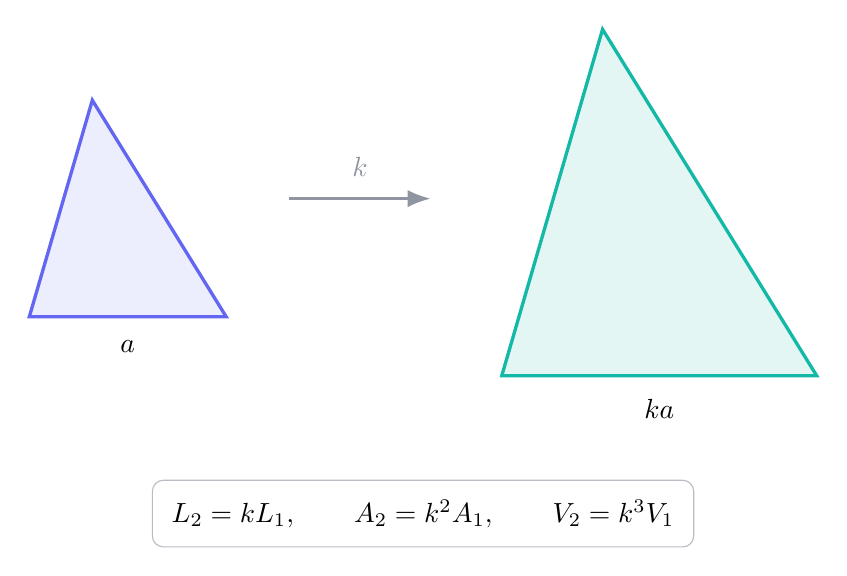
\begin{tikzpicture}[font=\sffamily,>=Latex]
  \fill[nebula!12] (-4,-1.5)--(-1.5,-1.5)--(-3.2,1.25)--cycle;
  \draw[very thick,nebula] (-4,-1.5)--(-1.5,-1.5)--(-3.2,1.25)--cycle;
  \node[below=5pt] at (-2.75,-1.5) {$a$};
  \draw[->,very thick,ink!55] (-.7,0)--(1.1,0) node[midway,above=4pt] {$k$};
  \fill[spark!12] (2,-2.25)--(6,-2.25)--(3.28,2.15)--cycle;
  \draw[very thick,spark] (2,-2.25)--(6,-2.25)--(3.28,2.15)--cycle;
  \node[below=5pt] at (4,-2.25) {$ka$};
  \node[draw=ink!35,rounded corners=4pt,fill=white,inner sep=7pt] at (1,-4)
    {$L_2=kL_1,\qquad A_2=k^2A_1,\qquad V_2=k^3V_1$};
\end{tikzpicture}
\end{document}
